\documentclass[a4paper,10pt]{article}
\usepackage[utf8]{inputenc}
\usepackage{amsmath}
\usepackage{xfrac}
%\usepackage[demo]{graphicx}
\usepackage[caption = false]{subfig}
\usepackage{float}
\usepackage[a4paper, total={7.5in, 11in}]{geometry}
\usepackage{longtable}
\usepackage{dcolumn,booktabs}
\usepackage[table]{xcolor}
\usepackage{listings}
\lstset{
breaklines=true
}
%http://tex.stackexchange.com/questions/116534/lstlisting-line-wrapping
\usepackage{hyperref}
\hypersetup{
    colorlinks=true,
    linkcolor=blue,
    citecolor=blue
}

\lstset{language=[77]Fortran,
  basicstyle=\ttfamily,
  keywordstyle=\color{red},
  commentstyle=\color{green},
  morecomment=[l]{!\ }% Comment only with space after !
}

\usepackage{color}
 
\definecolor{codegreen}{rgb}{0,0.6,0}
\definecolor{codegray}{rgb}{0.5,0.5,0.5}
\definecolor{codepurple}{rgb}{0.58,0,0.82}
\definecolor{backcolour}{rgb}{0.95,0.95,0.92}
 
\lstdefinestyle{mystyle}{
    backgroundcolor=\color{backcolour},   
    commentstyle=\color{codegreen},
    keywordstyle=\color{magenta},
    numberstyle=\tiny\color{codegray},
    stringstyle=\color{codepurple},
    basicstyle=\footnotesize,
    breakatwhitespace=false,         
    breaklines=true,                 
    captionpos=b,                    
    keepspaces=true,                 
    numbers=left,                    
    numbersep=5pt,                  
    showspaces=false,                
    showstringspaces=false,
    showtabs=false,                  
    tabsize=2
}
 
\lstset{style=mystyle}

%opening

\title{Homework 5 \\
\textbf{Laplace equation problem in 2D}}
\author{Arvind Balasubramanian}
\date{}

\begin{document}
\maketitle
\begin{lstlisting}[language=python]
import numpy as np

h = 10**(-1)
x = np.arange(0,2+h,h)
y = np.arange(0,1+h,h)
V = np.zeros((len(x), len(y)))
# Boundary Conditions
V[np.where(x==2),:] = 1
V[np.where(x==0),:] = -1
V[:,np.where(y==0)] = -1
V[:,np.where(y==1)] = 1
V_new = np.copy(V)
steps = 1000
s = 0

def partialx(V,x0,y0,stepsize):
    return (V[x0 + stepsize, y0] - V[x0 - stepsize, y0])/(2.0*stepsize) 

def partialy(V,x0,y0,stepsize):
    return (V[x0, y0 + stepsize] - V[x0, y0 - stepsize])/(2.0*stepsize)

while(s <= steps):
    s += 1
    for i in range(1,(len(x)-1)):
        for j in range(1,(len(y)-1)):
            V_new[i,j] = (1.0/4.0)*(V[i+1,j] + V[i-1,j] + V[i,j+1] + V[i,j-1])
            V = V_new
# Calculating E field            
for i in range(1,len(x)-1):
    for j in range(1,len(y)-1):
        Ex, Ey = np.meshgrid(-partialx(V,i,j,1),-partialy(V,i,j,1))
\end{lstlisting}

\begin{figure}[H]
\centering
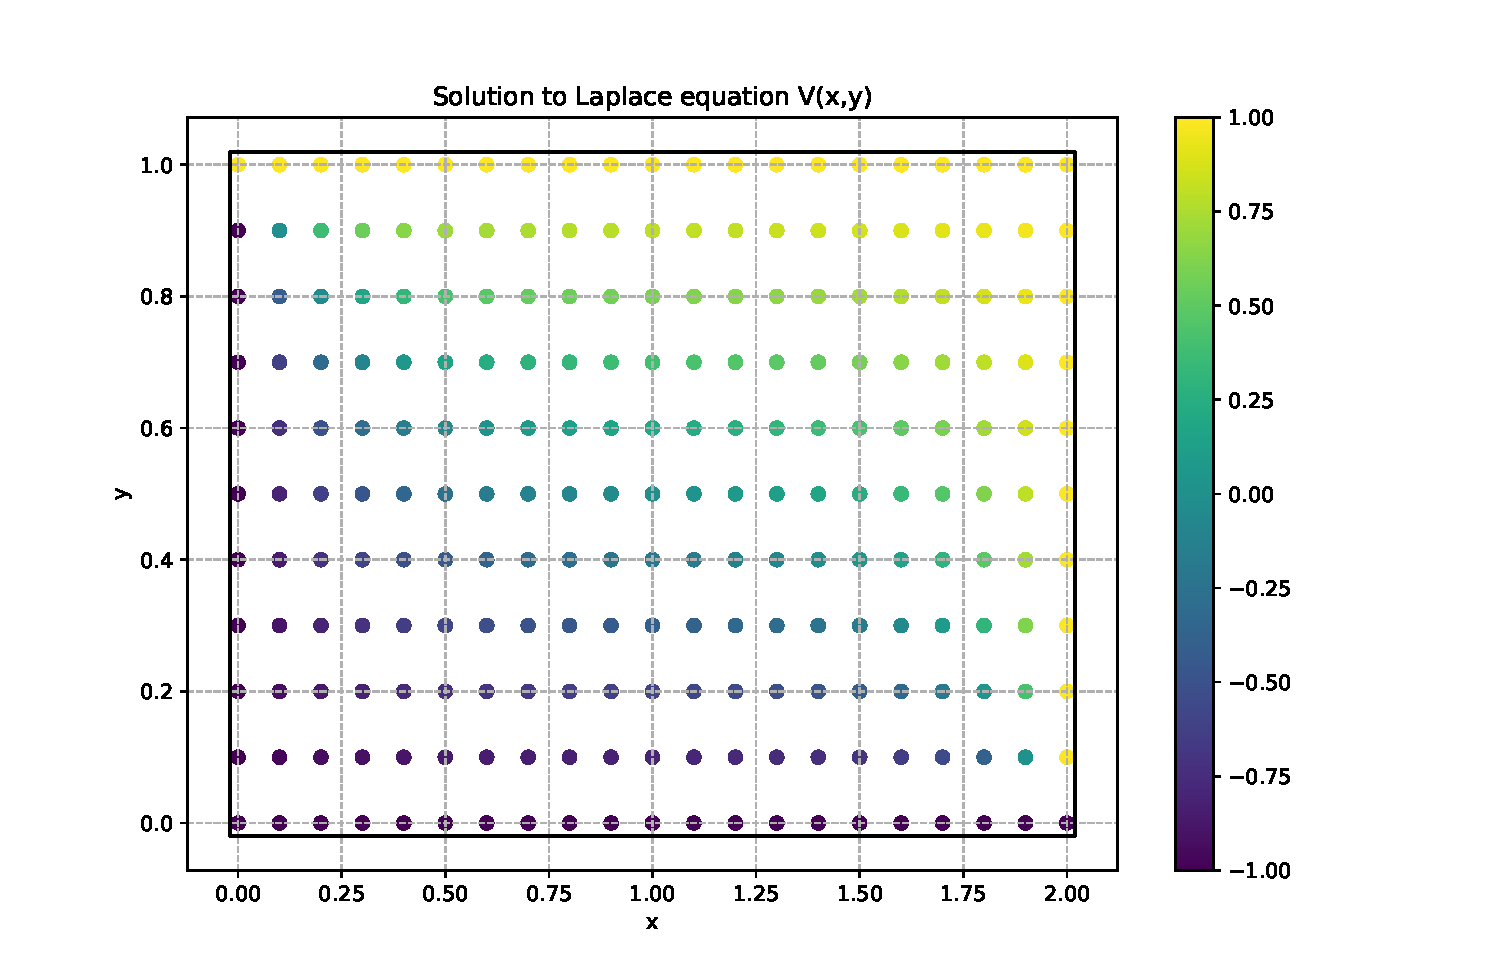
\includegraphics[scale=0.45]{solution} 
\end{figure}


\end{document}
